\section{Background}

% TODO section intro

\subsection{Basic terms}

\paragraph{Policy}
The IT portfolio of many current enterprises consists of a variety of different applications and systems. As a fine grained control of users' access to these resources is required, management of access rights for every user can become tedious. A set of rules is usually in place, which specify how a \textit{subject} (a person, user, actor) can interact with an \textit{object} (system, program), describing subject's accountability and capabilities within the object~\cite{Feltus2008PreliminaryConcept}. Policies are often used in the \hyperref[sec:xacml]{XACML} context.

\paragraph{Assertion}
An assertion is a ``confident and forceful statement of fact or belief''\footnotemark. In the context of authentication and in particular \hyperref[sec:saml]{SAML}, it is often the case that the identity provider is an independent entity, logically and physically separated from the application/relying party that requested user authentication. After the identity provider authenticates the user, it issues an assertion, confirming that the user's identity has been verified.

\footnotetext{\url{https://en.oxforddictionaries.com/definition/assertion}, accessed 05 March 2019}

\subsection{XACML}

 \acrfull{xacml} is a standardised, XML-based language for expressing security policies. It provides methods to define and combine security policies and to rapidly identify, which policy applies to a given subject. \acrshort{xacml} was first standardised by OASIS\footnote{\url{https://www.oasis-open.org/}, accessed 04 March 2019} in 2003 and the latest version is XACML 3.0, standardised in 2013~\cite{OASISStandard2013EXtensible3.0}. The further description is based on this latest version.
 
 The context of \acrshort{xacml} is illustrated in Figure~\ref{fig:xacml-context}. At the centre of the system is the \acrfull{pdp} which evaluates an input (such as access requests) against a policy set and issues an output -- a decision (such as \textit{access granted}). \acrshort{xacml} defines the formal language of the policy set and of the requests/responses. A policy set contains comprises one or more \textit{policies} and a \textit{policy combining algorithm}. The main components of a policy are a \textit{target} to which this policy applies and one or more \textit{rules}. The rule must specify a \textit{target} to which it applies and an \textit{evaluation} (\textit{permit} or \textit{deny}). It can also optionally specify \textit{conditions}, \textit{obligations} and \textit{advices}, all of which further shape the scope of the rule. Policy combining algorithm specifies the order and other conditions that decide, which policy will be finally applied on the request~\cite{OASISStandard2013EXtensible3.0}.
 
 \begin{figure}[ht]
    \centering
    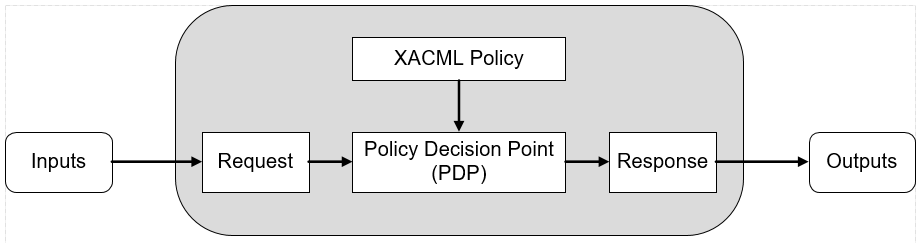
\includegraphics[width=.95\textwidth]{xacml-context}
    \caption{The context diagram of \acrshort{xacml}. From~\cite{OASISStandard2013EXtensible3.0}, edited.
    }
    \label{fig:xacml-context}
\end{figure}
 
The \acrshort{xacml} standard defines in detail several logical entities and their interactions. The native format for messages between these entities is XML, but a profile has been developed to support JSON message format~\cite{2017JSON1.0}. Additional profile was also created to describe implementation in a RESTful architecture~\cite{2017REST1.0}.
 
 Several implementations of \acrshort{xacml} exist in Java, Python and other languages. Criticisms of \acrshort{xacml} include low adoption rate, unsuitability for federated enterprises~\cite{Cser2013XACMLDead}, and lack of transparency for the end user~\cite{Cser2013XACMLDead, Ardagna2011ExpressiveApplications}.


\subsection{SAML}\label{sec:saml}

The \acrfull{saml} is a framework for exchange of assertions containing security information between two online parties, typically an identity provider and a relying party. Similarly as XACML, \acrshort{saml} was developed by OASIS. Version 1.0 was released in 2002 and version 2.0 (latest) in 2005. The rest of this report refers to version 2.0.

The main premise of \acrshort{saml} is that the \acrfull{idp} and the protected resource/application are two separated entities. This is desired, since it enables us to manage identities centrally for multiple applications and avoids duplication user accounts across these applications. Moreover, separating these enables both parts to specialise only in their task.

The Figure~\ref{fig:saml-architectire} illustrates the separation of these two entities. It also depicts the high-level flow of the authentication process. If the user wants to access the protected resource on the right, they first need to authenticate themselves with the \acrshort{idp}.

Another noteworthy aspect of \acrshort{saml} is the identity federation. This is achieved, when the \acrshort{idp} and the \acrshort{rp} are in different security realms, possibly operated by different organisations. As long as an agreement is established between the two, users can use identity managed by the \acrshort{idp} to access any resources outside the organisation's boundary~\cite{2008SecurityOverview}.

 \begin{figure}[ht]
    \centering
    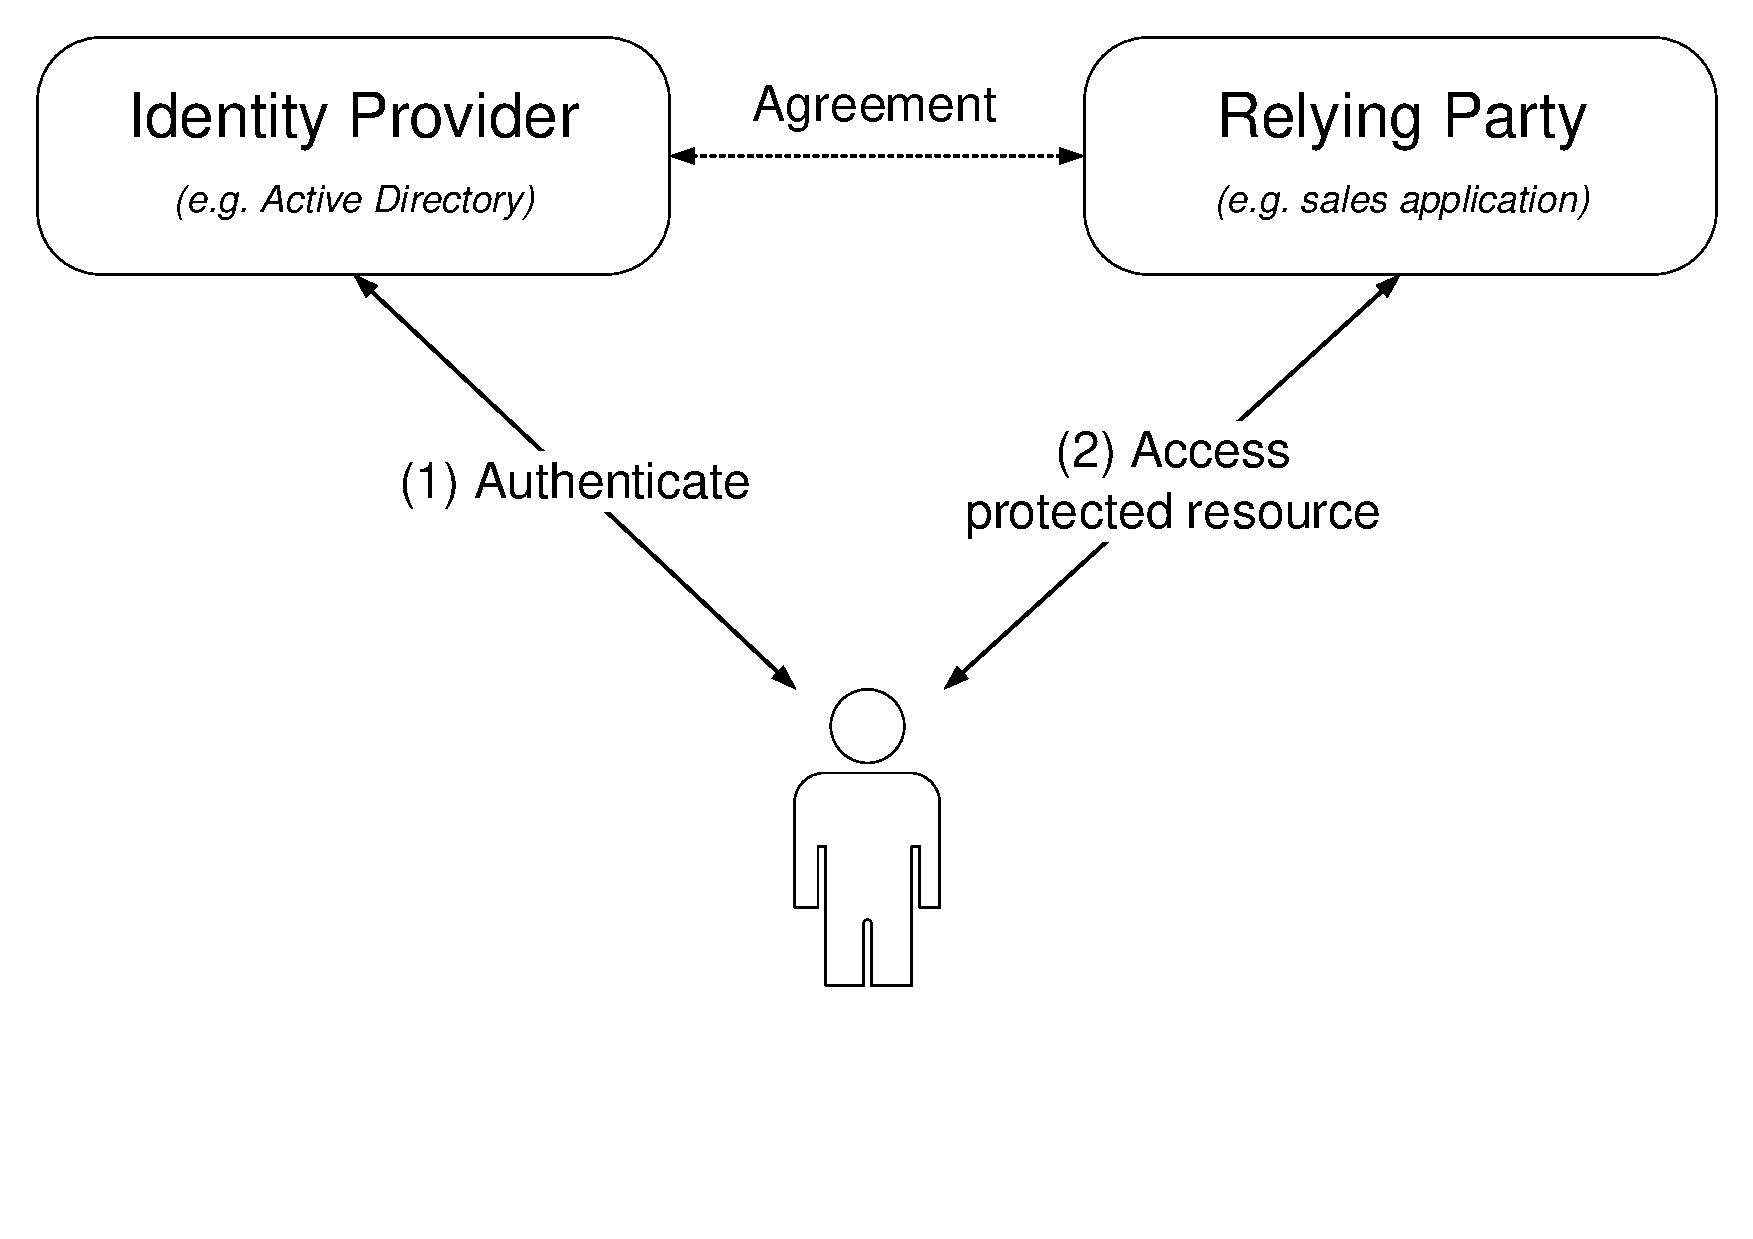
\includegraphics[width=.95\textwidth]{saml-architecture}
    \caption{The general use case of SAML, demonstrating the premise of functional separation of \acrshort{idp} and \acrshort{rp}. Taken from~\cite{2008SecurityOverview}.}
    \label{fig:saml-architectire}
\end{figure}

\paragraph{Assertions}
An assertion in \acrshort{saml} contains some security information about the \textit{subject}. Subject could be the user Bob and the associated information could be Bob's email address and job title. The security information need to be of one of following three categories:

\begin{enumerate*}[label=(\roman*)]
    \item \textit{Authentication statements} describe means and the timestamp of the authorisation carried out by the asserting party;
    \item \textit{Attribute statements} provide information about the subject; and
    \item \textit{Authorisation decision statement} describes what the subject is permitted to access in the system.
\end{enumerate*}

% \paragraph{Protocols}
% \acrshort{saml} defines a number of general protocols to facilitate the message exchange during different parts of the assertion process.

\paragraph{Bindings}
\acrshort{saml} describes how the messages exchanged during an assertion process can be bound to lower-level transport protocols. There are in total 6 bindings defined by the standard, but the following three are of particular interest:

\begin{itemize}[noitemsep]
    \item \textit{HTTP Redirect Binding}, where the entire \acrshort{saml} message is carried in the URL parameters, in the header of an HTTP GET method. This is suitable for short messages as the length of URL is limited in practice. This binding can be used in a RESTful system.
    \item \textit{HTTP POST Binding}, where the \acrshort{saml} message is base64 encoded into an XHTML form and transmitted using the HTTP POST method. This binding can also be used in a RESTful system.
    \item \textit{SAML SOAP Binding} specifies how the \acrshort{saml} messages are carried in an XML envelope over SOAP over any underlying transport protocol~\cite{Cantor2005BindingsV2.0}.
\end{itemize}

% \paragraph{Profiles}
% Several profiles which build on assertions and bindings are defined in the standard which correspond to the most common use cases of \acrshort{saml}. 

While \acrshort{saml} is widely adopted in the industry and is considered generally secure, numerous security flaws have been identified over time. Most of these arised from improper implementation of the protocol and have been patched since discovery~\cite{Krawczyk2014SecureAttacks}. The vulnerabilities included XML signature wrapping, assertion eavesdropping~\cite{Chen2014Environment-BoundAssertions} and XML parsing issues~\cite{Degges2018AVulnerability}.
